\chapter{Problem 1}
\section{Outline of solution}

The problem asks to find the length of the segment X1X2 in terms of R, where X1 and $X2$ are two points on a circle of radius R such that the 
angle $\alpha$ subtended by the chord X1X2 at the center of the circle satisfies the equation 
$$\alpha - sin(\alpha) =\frac{\pi}{2}$$.

\noindent To solve the problem, we first need to find the value of $\alpha$ that satisfies the equation. Unfortunately, there is no algebraic expression for $\alpha$ in terms of elementary functions, so we have to use numerical methods to approximate its value. One common method is the Newton-Raphson method, which involves starting with an initial guess for $\alpha$ and then iteratively improving the guess until it converges into a solution.


\section{CRC Model}
    \begin{center}
        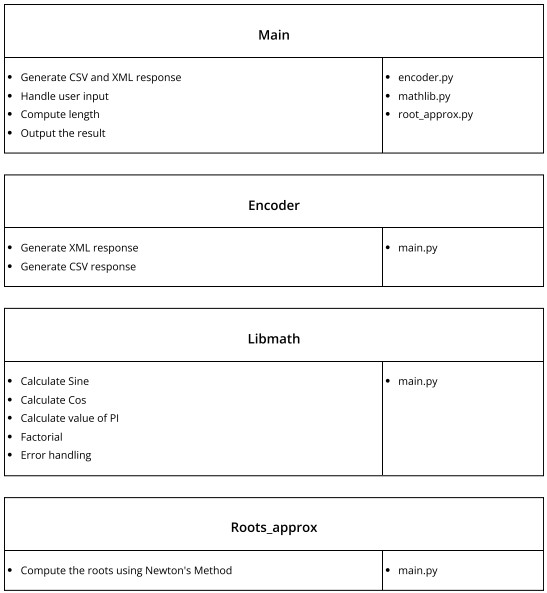
\includegraphics[width=10cm]{images/CRC_D1_Updated.jpg}
    \end{center}